\documentclass[12pt]{article}
\usepackage{amsmath}
\usepackage[utf8]{inputenc}
\usepackage[english, russian]{babel}
\usepackage[T2A]{fontenc}
\usepackage{graphicx}
\usepackage{float}
\usepackage[top=1in, bottom=1.25in, left=1.25in, right=1.25in]{geometry}
\title{\LaTeX}
\date{}
\begin{document}

\def\dd#1#2{\frac{\partial#1}{\partial#2}}

{\large УДК 004.8}
\part*{Нейросетевый метод снятия омоним}
Нгуен Нгок Дьеп, Ле Мань Ха - Московский Физико-Технический Институт

\section{Введение}

В лексической системе русского языка есть слова, которые звучат одинаково, но имеют совершенно разные значения. Такие слова называются лексическими омонимами, а звуковое и грамматическое совпадение разных языковых единиц, которые семантически не связаны друг с другом, называется омонимией \cite{Homonym}.

Например:
\begin{itemize}
\item[1.] Ключ(1) – «Родник» (Студеный ключ)
\item[] Ключ(2) – Стальной ключ для отпирания и запирания замка
\item[2.] Лук(1) – «Растение» зеленый лук
\item[] Лук(2) – «оружие» тугой лук
\end{itemize}

В отличие от многозначных слов лексические омонимы не обладают предметно-семантической связью, т.е. у них нет общих семантических признаков, по которым можно было бы судить о полисемантизме одного слова. Полная лексическая омонимия – это совпадение слов, принадлежащих к одной части речи, во всех формах. Пример: наряд(1) – «одежда», наряд(2) – «распоряжение»; Замок(1) – «123», Замок(2) – «здание»;

Автоматическая система перевода делится на несколько этапов, одним из которых является морфологический. На этом этапе для каждого слова определяются морфологические характеристики: род, число, падеж, склонение, и т.п., а также начальная форма слова (Лемма). Процесс морфологической разметки осложняется омонимами \cite{Homonym}.
\section{Методы представления текста}
	В настоящее время теория и практика машинного обучения переживают настоящую «глубинную революцию», вызванную успешным применением методов deep learning, представляющих собой третье поколение нейронных сетей. Сети, обученные с помощью алгоритмов глубинного обучения, не просто превзошли по точности лучшие альтернативные подходы, но и в ряде задач проявили зачатки понимания смысла подаваемой информации (например, при распознавании изображений, анализе текстовой информации и т.п.). Наиболее успешные современные промышленные методы компьютерного зрения, распознавания речи и машинного перевода построены на использовании глубинных сетей, а гиганты IT-индустрии, такие как Apple, Google, Facebook, скупают коллективы исследователей, занимающихся глубинным обучением целыми лабораториями.

Представление слова как вектор - в настоящее время одна из самых интересных областей исследований в глубинном обучении, хотя данный подход был изначально введен Bengio \cite{Bengio} и др. более десяти лет назад.

	Самый известные модели представления слова как вектор представлены Mikolov (2013a)\cite{Mikolov} и реализация моделей Word2vec \cite{word2vec} опубликована на сайте Google project, которая привлекла большое внимание в последние два года – это “Continuous-Bag-of-Word” и “Skip-Gram”. Эти модели использовали простую нейронную сеть для отображения слов, которые ближе к слову по значению. Поэтому процесс обучения для этих моделей быстро работает с большими данными. 
	
	\begin{figure}[H]
		\noindent\centering{
			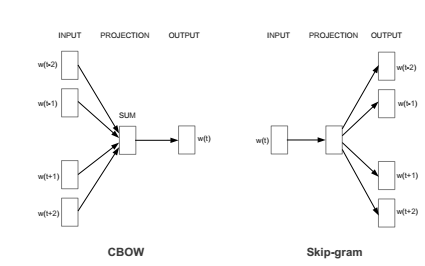
\includegraphics[width=90mm]{cbow.png}	
		}
		\caption{Модели CBOW и Skip-gram.}
		\label{figCurves}
	\end{figure}
	
CBOW модель – Использует окружающие слова (предложение без заданного слова), что бы предугадать заданное слово. Входные вектора в нейронную сеть W(t-2),W(t-1), W(t+1), W(t+2), а выходной вектор из сети это заданное слово W(t). В результате обучения получается 2 вектора представления слова. Входной вектор V - это вектор представления предложения описания слова, выходной вектор V’ – Это вектор представления слова.

SKIP-GRAM модель – Использует слово, что бы предугадать предложение описания заданного слова.

 	\begin{figure}[H]
		\noindent\centering{
			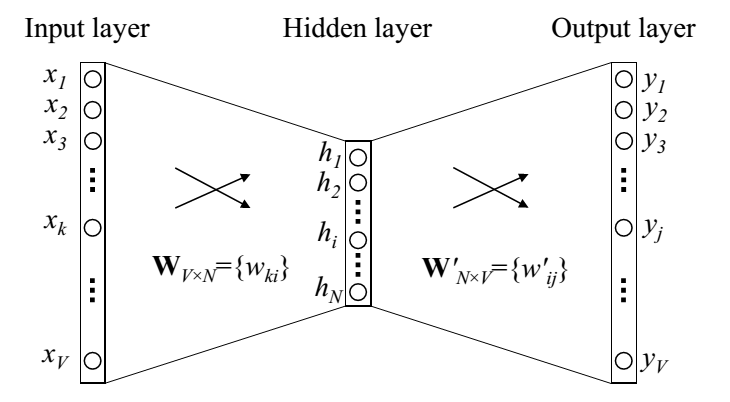
\includegraphics[width=90mm]{cbow2.png}	
		}
		\caption{Показал нейронную сеть, использованную чтобы получить вектор представления слова. Входной слой и выходной имеют V нейронов, а скрыты имеет N нейронов.}
		\label{figCurves}
	\end{figure}

Эти модели могут использоваться во многих задачах анализа естественного языка, таких как классификация документов, распознавание спама или машинный перевод.

На рисунке 3, визуализировали векторы для чисел и животных на английском и испанском языках \cite{Le}, и он может быть легко видеть, что эти понятия имеют схожие геометрические композиции. Причина в том, что, как и все распространенные языки поделиться понятия, которые основаны на реальном мире.
	\begin{figure}[H]
		\noindent\centering{
			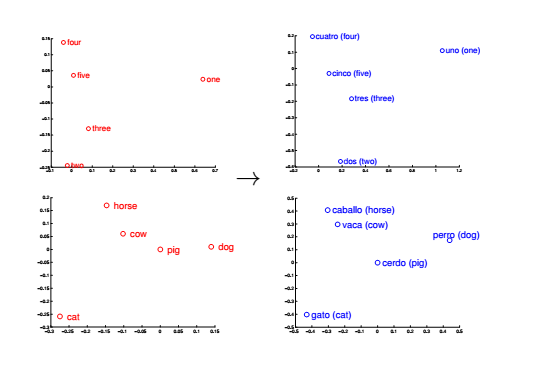
\includegraphics[width=140mm]{translate2.png}	
		}
		\caption{Распределенная векторных представлений слов чисел и животных на английском языке (слева) и испанском (справа).пять Векторов на каждом языке были спроектированы до двух измерениях с использованием РСА. Видно, что эти концепции имеют схожие механизмы геометрические в обоих пространствах, предполагая, что можно узнать точную линейное отображение из одного пространства в другое.}
		\label{figCurves}
	\end{figure}

Один хороший пример это двуязычный слово вложение, производится в Socher др. (2013a)\cite{Zou}. Мы можем научиться вставлять слова из двух разных языков в одной общей пространстве. В этом случае, мы учимся вставлять английские и китайский слов в том же пространстве.

Одна вещь, мы можем сделать, чтобы почувствовать слова вложения пространства для визуализации их трет-СНЭ, сложной техники для визуализации многомерных данных

 	\begin{figure}[H]
		\noindent\centering{
			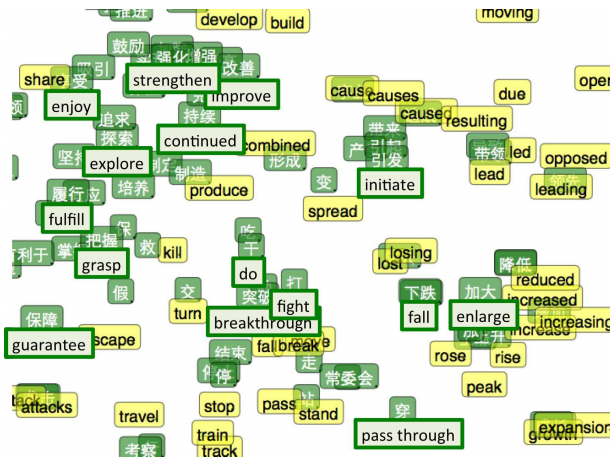
\includegraphics[width=100mm]{translate.png}	
		}
		\caption{Английский и китайский язык.}
		\label{figCurves}
	\end{figure}

	

Таким образом, возможно снять омонимию через окружающие слова в предложении. Если значение слов окружающих омонимы разные, тогда расстояние между омонимами тоже большое.

\section{Нейронные сети и Автоэнкодер}

Нейронные сети прямого распространения часто используются для обучения с учителем и используются, например, для классификации \cite{Stanford1}.

  \begin{figure}[H]
    \noindent\centering{
        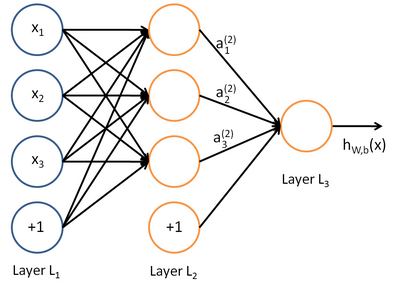
\includegraphics[width=100mm]{mnn.png}
    }
    \caption{Многослойная нейронная сеть}
    \label{figCurves}
  \end{figure}

Часто используемая функция активации - сигмоид:
  \begin{align}
	f(z_j)=\sigma(z_j)=(1+e^{-z_j})^{-1}
  \end{align}

Где:

  \begin{align}
	z_j=\sum{{w_{ij}}{x_i}}
  \end{align}

Полезное свойство сигмоида - её производная функции:
  \begin{align}
	\dd{\sigma}z=\sigma(z)(1-\sigma(z))
  \end{align}

Обучение такой нейронной сети производится обычно методом обратного распространения ошибки таким образом, чтобы минимизировать среднеквадратическую ошибку сети на обучающей выборке. Таким образом, обучающая выборка содержит пары векторов признаков (входные данные) и эталонных векторов (маркированные данные) {(x, y)}.

Метод обратного распространения ошибки:

Для выходного нейрона:
  \begin{align}
	\delta=z-y
  \end{align}

Для нейронов скрытых слоев:
  \begin{align}
	\delta_i=\sum_{j=0}^n \delta_j w_{ij}
  \end{align}

Коррекция весов:

Для выходного нейрона:
  \begin{align}
	w_{i0}'=w_{i0}+\eta\delta y_i
  \end{align}

Для нейронов скрытых слоев:
  \begin{align}
	w_{ij}'=w_{ij}+\eta\delta_j y_j(1-y_j)y_i
  \end{align}

В реальной практике, маркированных данных очень мало, для них требуется много сил и времени. Автоэнкодер представляет собой алгоритм обучения без учителя, который использует нейронную сеть и метод обратного распространения ошибки для того, чтобы добиться того, что входной вектор признаков вызывал выход сети, равный входному вектору, т.е. y = x.

Автоэнкодер явлается специальной архитектурой искусственных нейронных сетей, позволяющая применять обучение без учителя при использовании метода обратного распространения ошибки. Простейшая архитектура автоэнкодера — сеть прямого распространения, без обратных связей, наиболее схожая с перцептроном и содержащая входной слой, скрытый слой и выходной слой. В отличие от перцептрона, выходной слой автоэнкодера должен содержать столько же нейронов, сколько и входной слой \cite{Stanford2}.

  \begin{figure}[H]
    \noindent\centering{
        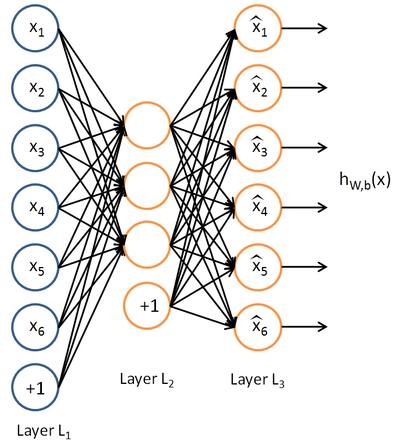
\includegraphics[width=100mm]{autoencoder.png}
    }
    \caption{Автоэнкодер}
    \label{figCurves}
  \end{figure}

Цель автоэнкодер - чтобы выход нейронной сети был наиболее близким к входному вектору. Для того, чтобы решение этой задачи было нетривиальным, на топологию сети накладываются особые условия:

1. Количество нейронов скрытого слоя должно быть меньше, чем размерность входных данных.

2. Активация нейронов скрытого слоя должна быть разреженной.

Первое ограничение позволяет получить сжатие данных при передаче входного сигнала на выход сети. Такая сжатие возможно, если в данных есть скрытые взаимосвязи, корреляция признаков или структура.

Второе ограничение – требование разреженной активации нейронов скрытого слоя, — позволяет получить нетривиальные результаты даже когда количество нейронов скрытого слоя превышает размерность входных данных. Будем считать нейрон активным, когда значение его функции передачи близко к 1 и наоборот, неактивным если значение его функции передачи близко к 0. Разреженная активация – это когда количество неактивных нейронов в скрытом слое значительно превышает количество активных.

Эти ограничения заставляют нейросеть искать обобщения и корреляцию в поступающих на вход данных, выполнять их сжатие. Таким образом, нейросеть автоматически обучается выделять из входных данных общие признаки, которые кодирутся в значениях весов сети.

Мы хотим, чтобы средняя активация каждого скрытого нейронна приняла значение, наиболее близкое к заданному разреженному параметру (порядка 0.05). Для этого, мы добавим в каждый нейрон скрытого слоя параметр разреженности $\rho$:

  \begin{align}
	\hat \rho_j=\frac{1}{m}\sum_{i=1}^m\biggl[a^{(2)}_j(x^{(i)})\biggl]
  \end{align}

  Мы хотим, чтобы средняя активация каждого скрытого нейронна приняла значение, наиболее близкое к $\rho$:
  \begin{align}
	\hat \rho_j=\rho
  \end{align}
  Штравная функция:
  \begin{align}
	S=\sum_{j=1}^{s_2}{KL({\rho}|{\hat{\rho_j}})}\\
	KL({\rho}|{\hat{\rho_j}})=\rho\log{\frac{\rho}{\hat{\rho_j}}}+(1-\rho)\log{\frac{1-\rho}{1-\hat{\rho_j}}}
  \end{align}
  Производная штравной функции:
  \begin{align}
	\dd{KL({\rho}|{\hat{\rho_j}})}{\rho_j}=-\frac{\rho}{\hat{\rho_j}} + \frac{1-\rho}{1-\hat{\rho_j}}
  \end{align}

\section{Рекурсивный автоэнкодер и векторное представление текста}

В данном разделе посмотрим как представит текст в виде числового вектора. Для решения классификации и других задач с помощью нейронных сетей, вход должен иметь фиксированную длину, а длинна текста явлается произвольной. Для фиксирования размера входов нейронных сетей используется метод векторного представления текста с помощью рекурсивного автоэнкода - входной и выходной слои которого имеют 2K нейронов, а скрытый слой - K нейронов \cite{Socher2}: 

Автоэнкодер объединяет два слова x1, x2 (вектор длины 2K) в один вектор y (длина К):

  \begin{align}
	y=f{(W^{(1)}[x1, x2] + b^{(1)})}
  \end{align}

Этот процесс повторяется N-1 раз для текта длинной N. В результате получается конечный вектор - семантическое векторное представление текста, этот вектор используем как вход для системы обучения.

  \begin{figure}[H]
    \noindent\centering{
        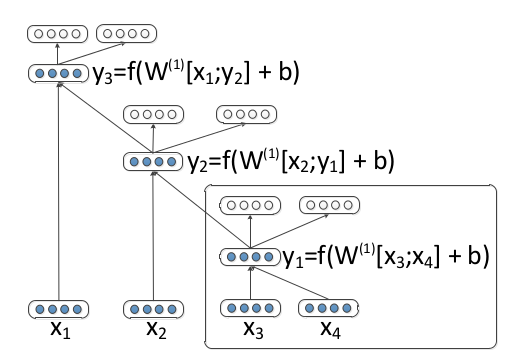
\includegraphics[width=120mm]{RAE.png}
    }
    \caption{Автоэнкодер}
    \label{figCurves}
  \end{figure}

\section{Кластеризация значений слова}

\subsection{K-means}

K-means - наиболее популярный метод кластеризации. Был изобретён в 1950-х годах математиком Гуго Штейнгаузом и почти одновременно Стюартом Ллойдом. Особую популярность приобрёл после работы Маккуина. Действие алгоритма таково, что он стремится минимизировать суммарное квадратичное отклонение точек кластеров от центров этих кластеров \cite{kmeans}:

	\begin{align}
		J(V) = \sum_{j}^{c}\sum_{j}^{c_i}(x_i-v_i)^2
	\end{align}

Следующим шагом является принятие каждую точку, принадлежащую к данному набору данных и связать его в ближайший центр. В этот момент мы должны пересчитать К новые центра, как барицентра кластеров в результате предыдущего шага. После того как мы вычислим эти новые К центроиды, новую привязку должно быть сделано между теми же набора данных точек и ближайшей нового центра. Цикл был сформирован. В результате этого цикла можно заметить, что K-центры меняют шаг за шагом местоположения пока больше изменений не сделано или, другими словами центры не двигаться больше.

	

\subsection{Маркировка значений слова}

В первых получить все возможные вектора слов, затем вектора используются, чтобы построить вектора контекстов с применением автоэнкодер[Session 4].

Например у нас есть миллион векторов описания о слове Замок, необходимо Выпольнять вычисления по алгоритму К-Means для этих веторов. В результате, мы сможем маркировать кождое слово с  значением.

Таким образом, все омонимs будут маркированы по значению, мы сможем использавать эти резутаты длы задачи снятия омонимий. 

\begin{thebibliography}{0}
\bibitem{Bengio}
Yoshua Bengio, Rejean Ducharme, Pascal Vincent, and Christian Jauvin. 2003. A neural probabilistic language model. In Journal of Machine Learning Research, pages 1137–1155.

\bibitem{Ruscorpora}
Национальный корпус русского языка, www.ruscorpora.ru

\bibitem{Socher1}
Richard Socher, John Bauer, Christopher D. Manning, and Andrew Y. Ng. 2013. Parsing with compositional vector grammars. In ACL.

\bibitem{Stanford1}
Stanford UFLDL tutorial, Multilayer neural networks 

http://ufldl.stanford.edu/tutorial/supervised/MultiLayerNeuralNetworks/

\bibitem{Stanford2}
Stanford UFLDL tutorial, Autoencoders

http://ufldl.stanford.edu/tutorial/unsupervised/Autoencoders/

\bibitem{Socher2}
Semi-Supervised Recursive Autoencoders for Predicting Sentiment Distributions, Richard Socher, Jeffrey Pennington, Eric H. Huang, Andrew Y. Ng, Christopher D. Manning, 2011

\bibitem{Le}
Mikolov, Tomas, Quoc V. Le, and Ilya Sutskever. "Exploiting similarities among languages for machine translation." arXiv preprint arXiv:1309.4168 (2013).

\bibitem{Zou}
Zou, W. Y., Socher, R., Cer, D. M., Manning, C. D. (2013). Bilingual Word Embeddings for Phrase-Based Machine Translation. In EMNLP (pp. 1393-1398)

\bibitem{Mikolov}
Mikolov, Tomas, et al. "Distributed representations of words and phrases and their compositionality." Advances in neural information processing systems. 2013.

\bibitem{Homonym} 
Омонимы в русском языке http://gramma.ru/

\bibitem{word2vec}
Word2Vec Project https://code.google.com/p/word2vec/

\bibitem{kmeans}
Алгоритм K-means https://ru.wikipedia.org/wiki/K-means

\end{thebibliography}

\end{document}
